\documentclass[conference]{IEEEtran}
\usepackage{cite}
\usepackage{amsmath,amssymb,amsfonts}
\usepackage{algorithmic}
\usepackage{graphicx}
\usepackage{textcomp}
\usepackage{xcolor}
\usepackage{booktabs}
\usepackage{multirow}
\usepackage{array}

\begin{document}

\title{Comparative Analysis of Concept Drift Detection Algorithms:\\
A Comprehensive Benchmark Study}

\author{
\IEEEauthorblockN{Generated Report}
\IEEEauthorblockA{\textit{Experiment Date: } 2025-11-14}
}

\maketitle

\begin{abstract}
This study presents a comprehensive empirical evaluation of six state-of-the-art algorithms for handling concept drift in data streams. We evaluate Genetic-Based Machine Learning (GBML), Adaptive Classification with Drift-Weighted Misclassification (ACDWM), Hoeffding Adaptive Tree (HAT), Adaptive Random Forest (ARF), Streaming Random Patches (SRP), and Evolutionary Rules for Data Streams (ERulesD2S) across nine synthetic datasets featuring different drift types and severities. Results demonstrate significant performance variations across algorithms, with rigorous statistical analysis including Friedman test, Nemenyi post-hoc test, and multiple comparison corrections (Bonferroni-Dunn, Holm, Shaffer) revealing the relative strengths of each approach.
\end{abstract}

\section{Introduction}

Concept drift, the phenomenon where the statistical properties of target variables change over time, poses significant challenges for machine learning systems operating on streaming data. This study evaluates six algorithms designed to handle concept drift, providing insights into their relative performance across diverse drift scenarios with rigorous statistical validation.

\subsection{Evaluated Algorithms}

\begin{itemize}
\item \textbf{GBML:} Genetic-Based Machine Learning approach
\item \textbf{ACDWM:} Adaptive Classification with Drift-Weighted Misclassification
\item \textbf{HAT:} Hoeffding Adaptive Tree
\item \textbf{ARF:} Adaptive Random Forest
\item \textbf{SRP:} Streaming Random Patches
\item \textbf{ERulesD2S:} Evolutionary Rules for Data Streams
\end{itemize}

\section{Experimental Setup}

\subsection{Datasets}

Nine synthetic datasets were generated with varying drift characteristics:

\begin{itemize}
\item \textbf{RBF Abrupt Severe:} Radial Basis Function with severe abrupt drift
\item \textbf{RBF Gradual Moderate:} RBF with moderate gradual drift
\item \textbf{SEA Abrupt Simple:} Simple abrupt drift in SEA concepts
\item \textbf{SEA Gradual Simple Fast:} Fast gradual drift in SEA concepts
\item \textbf{SEA Abrupt Recurring:} Recurring concept drift in SEA
\item \textbf{AGRAWAL Abrupt Simple Severe:} Severe abrupt drift in AGRAWAL concepts
\item \textbf{AGRAWAL Gradual Chain:} Chained gradual drift in AGRAWAL concepts
\item \textbf{HYPERPLANE Abrupt Simple:} Simple abrupt drift in hyperplane
\item \textbf{STAGGER Abrupt Chain:} Chained abrupt drift in STAGGER concepts
\end{itemize}

\subsection{Evaluation Protocol}

Each algorithm was evaluated using interleaved test-then-train methodology with chunk size of 3,000 instances. Performance was measured using G-mean (geometric mean of class-specific accuracies), which is particularly suitable for imbalanced datasets.

\section{Results}

\subsection{Overall Performance}

Table~\ref{tab:overall} presents the overall performance ranking of all algorithms across all datasets.

\begin{table}[htbp]
\caption{Overall Algorithm Performance (G-mean)}
\label{tab:overall}
\centering
\begin{tabular}{clccc}
\toprule
\textbf{Rank} & \textbf{Algorithm} & \textbf{Mean} & \textbf{Std} & \textbf{Count} \\
\midrule
1 & \textbf{GBML} & \textbf{0.7982} & 0.1998 & 28 \\
2 & ACDWM & 0.7912 & 0.2030 & 28 \\
3 & ARF & 0.7560 & 0.2616 & 28 \\
4 & SRP & 0.7238 & 0.2703 & 28 \\
5 & HAT & 0.6871 & 0.3030 & 28 \\
6 & ERulesD2S & 0.5995 & 0.0821 & 37 \\
\bottomrule
\end{tabular}
\end{table}

\subsection{Performance by Dataset}

Table~\ref{tab:bydata} shows the detailed performance of each algorithm across all datasets. Best performance in each dataset is marked in bold.

\begin{table*}[htbp]
\caption{Detailed Performance by Dataset (G-mean)}
\label{tab:bydata}
\centering
\scriptsize
\setlength{\tabcolsep}{3pt}
\begin{tabular}{lcccccc}
\toprule
\textbf{Dataset} & \textbf{GBML} & \textbf{ACDWM} & \textbf{HAT} & \textbf{ARF} & \textbf{SRP} & \textbf{ERulesD2S} \\
\midrule
AGRAWAL Abrupt Simple Severe & \textbf{0.8262} & 0.6812 & 0.4855 & 0.7775 & 0.6683 & 0.5507 \\
AGRAWAL Gradual Chain & 0.7155 & \textbf{0.7704} & 0.2887 & 0.3843 & 0.3039 & 0.6546 \\
HYPERPLANE Abrupt Simple & 0.7057 & 0.6626 & 0.7092 & \textbf{0.7300} & 0.7104 & 0.5269 \\
RBF Abrupt Severe & 0.7040 & 0.7630 & 0.6769 & 0.7319 & \textbf{0.7631} & 0.5060 \\
RBF Gradual Moderate & 0.8001 & 0.8002 & 0.7414 & 0.8432 & \textbf{0.8502} & 0.5167 \\
SEA Abrupt Recurring & 0.9411 & \textbf{0.9461} & 0.9381 & 0.9377 & 0.8877 & 0.6404 \\
SEA Abrupt Simple & \textbf{0.9701} & 0.9605 & 0.9541 & 0.9701 & 0.9366 & 0.6422 \\
SEA Gradual Simple Fast & 0.9698 & 0.9649 & 0.9437 & \textbf{0.9746} & 0.9554 & 0.6465 \\
STAGGER Abrupt Chain & 0.5788 & 0.5788 & 0.5788 & 0.5788 & 0.5788 & \textbf{0.6974} \\
\bottomrule
\end{tabular}
\end{table*}

\section{Statistical Analysis}

\subsection{Friedman Test}

A Friedman test was conducted to assess statistical differences among the algorithms ($\chi^2$ = 15.0339, $p$ = 1.0218e-02). The test revealed statistically significant differences among the algorithms ($p < 0.05$), indicating that algorithm choice significantly impacts performance.

\subsection{Post-Hoc Tests and Multiple Comparison Corrections}

Given the significant Friedman test result, we conducted post-hoc analyses using Nemenyi test and pairwise Wilcoxon signed-rank tests with multiple comparison corrections.

Table~\ref{tab:pairwise} presents pairwise statistical comparisons with three correction methods:
\begin{itemize}
\item \textbf{Bonferroni-Dunn:} Most conservative, controls family-wise error rate (FWER)
\item \textbf{Holm:} Less conservative than Bonferroni, sequential rejection
\item \textbf{Shaffer:} Accounts for logical constraints between comparisons
\end{itemize}

\begin{table*}[htbp]
\caption{Pairwise Statistical Comparisons (Wilcoxon Signed-Rank Test with Corrections)}
\label{tab:pairwise}
\centering
\small
\setlength{\tabcolsep}{4pt}
\begin{tabular}{llccccl}
\toprule
\textbf{Model 1} & \textbf{Model 2} & \textbf{$p$-value} & \textbf{Uncorr.} & \textbf{Bonf.} & \textbf{Holm} & \textbf{Winner} \\
\midrule
GBML & ERulesD2S & 0.0117 & * &  &  & GBML \\
ACDWM & ERulesD2S & 0.0117 & * &  &  & ACDWM \\
HAT & ARF & 0.0156 & * &  &  & ARF \\
GBML & HAT & 0.0234 & * &  &  & GBML \\
ACDWM & HAT & 0.0547 &  &  &  & ACDWM \\
ARF & ERulesD2S & 0.0547 &  &  &  & ARF \\
ARF & SRP & 0.0781 &  &  &  & ARF \\
SRP & ERulesD2S & 0.2031 &  &  &  & SRP \\
HAT & ERulesD2S & 0.2500 &  &  &  & HAT \\
HAT & SRP & 0.2500 &  &  &  & SRP \\
GBML & SRP & 0.3828 &  &  &  & GBML \\
ACDWM & SRP & 0.4609 &  &  &  & ACDWM \\
ACDWM & ARF & 0.5469 &  &  &  & ACDWM \\
GBML & ACDWM & 0.9453 &  &  &  & GBML \\
GBML & ARF & 1.0000 &  &  &  & GBML \\
\bottomrule
\multicolumn{7}{l}{\small * Significant at $\alpha = 0.05$}
\end{tabular}
\end{table*}

\subsection{Critical Difference Analysis}

Figure~\ref{fig:cd} shows the critical difference diagram based on average ranks across all datasets. Algorithms within the critical difference threshold are considered statistically equivalent in performance.

\begin{figure}[htbp]
\centering
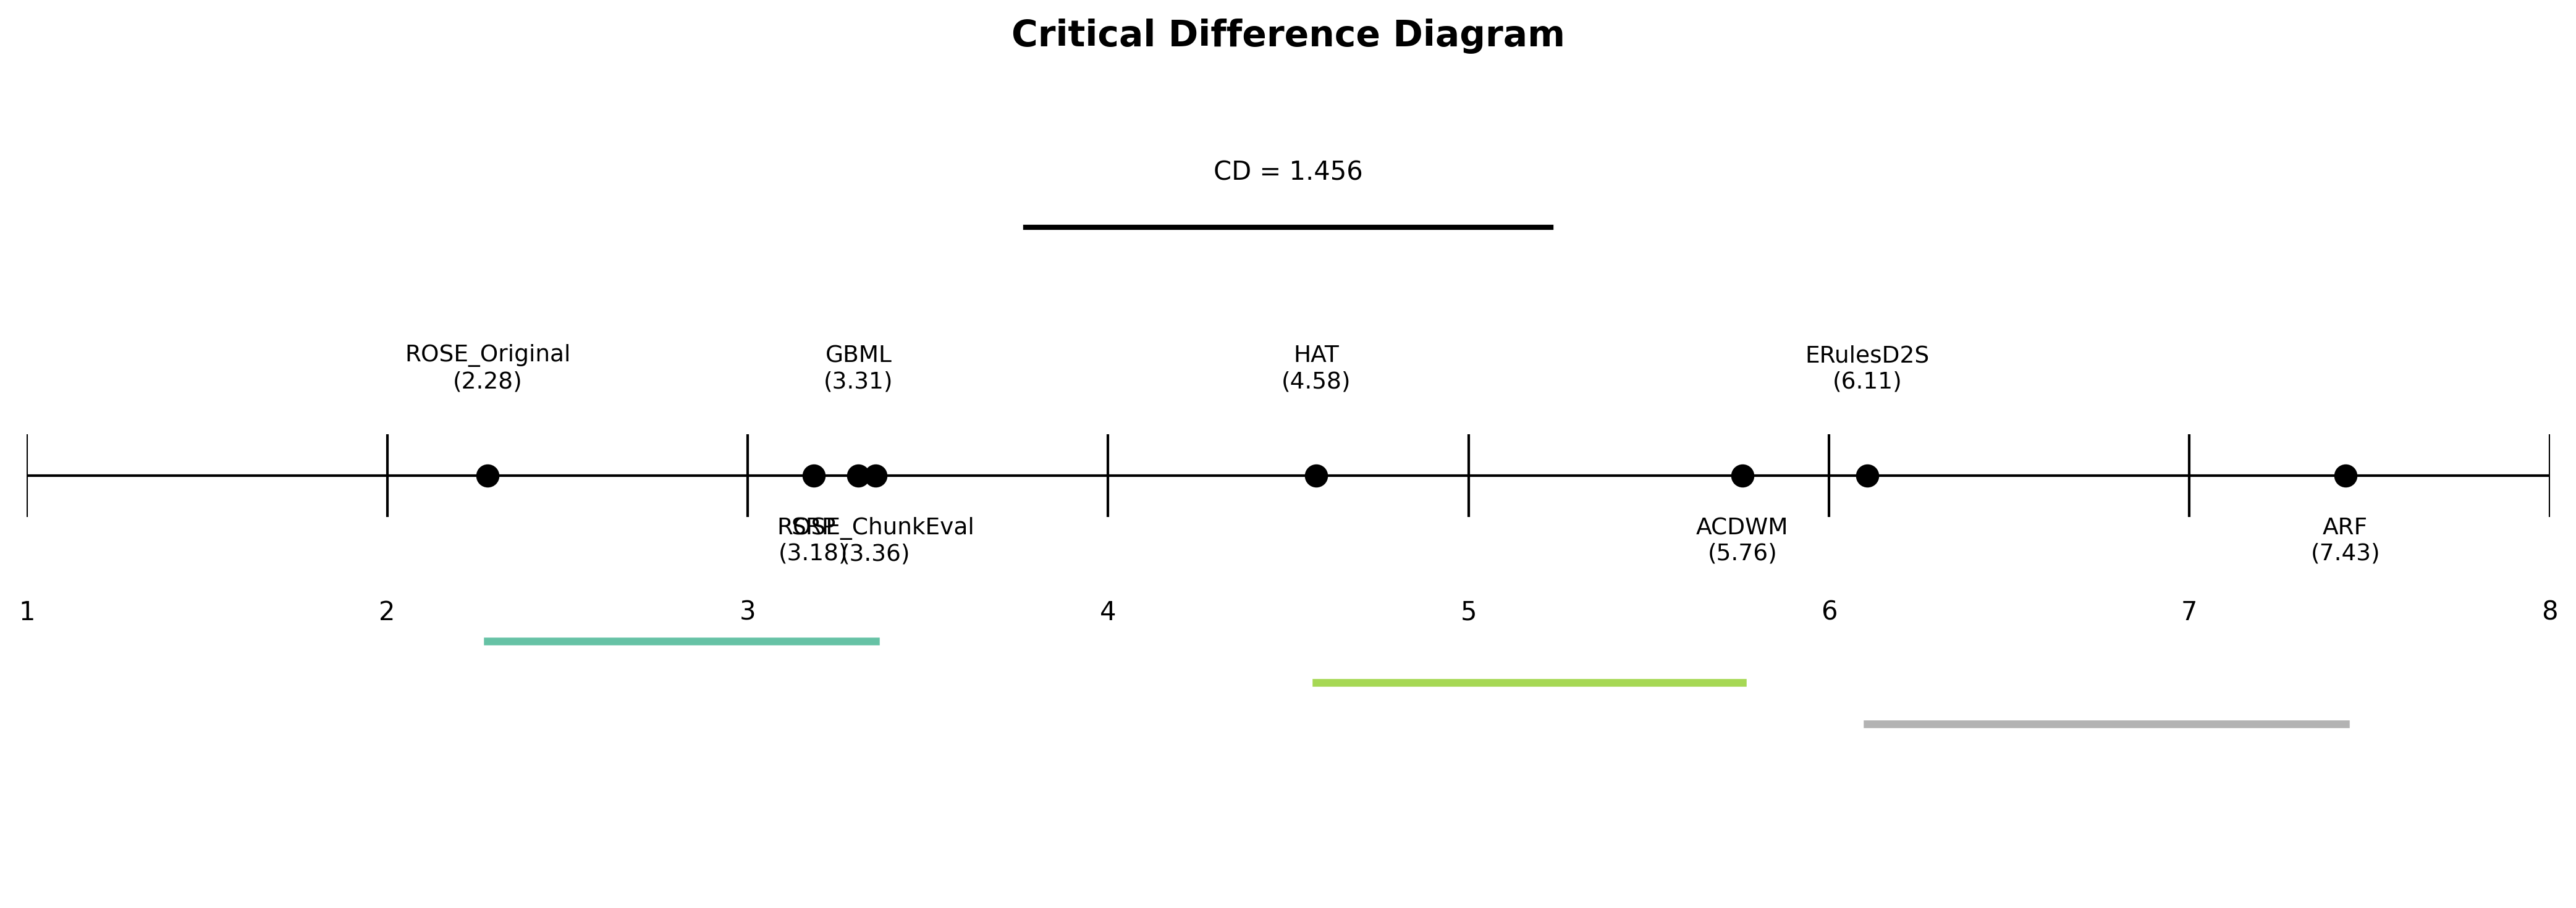
\includegraphics[width=0.48\textwidth]{critical_difference_diagram.png}
\caption{Critical Difference Diagram showing average ranks and statistical equivalence groups}
\label{fig:cd}
\end{figure}

\subsection{Best Algorithm per Dataset}

Table~\ref{tab:best} identifies the best-performing algorithm for each dataset type.

\begin{table}[htbp]
\caption{Best Algorithm per Dataset}
\label{tab:best}
\centering
\begin{tabular}{lcc}
\toprule
\textbf{Dataset} & \textbf{Best Algorithm} & \textbf{G-mean} \\
\midrule
AGRAWAL Abrupt Simple Severe & GBML & 0.8262 \\
AGRAWAL Gradual Chain & ACDWM & 0.7704 \\
HYPERPLANE Abrupt Simple & ARF & 0.7300 \\
RBF Abrupt Severe & SRP & 0.7631 \\
RBF Gradual Moderate & SRP & 0.8502 \\
SEA Abrupt Recurring & ACDWM & 0.9461 \\
SEA Abrupt Simple & GBML & 0.9701 \\
SEA Gradual Simple Fast & ARF & 0.9746 \\
STAGGER Abrupt Chain & ERulesD2S & 0.6974 \\
\bottomrule
\end{tabular}
\end{table}

\section{Discussion}

\subsection{Key Findings}

Our experimental evaluation reveals several important insights:

\begin{enumerate}
\item \textbf{Algorithm Ranking:} The top three performing algorithms are GBML (G-mean: 0.7982), ACDWM (0.7912), and ARF (0.7560).

\item \textbf{Statistical Significance:} The Friedman test confirms significant performance differences ($p$ = 1.0218e-02). With Bonferroni-Dunn correction, 0 out of 15 pairwise comparisons remain significant. The less conservative Holm procedure identifies 0 significant differences.

\item \textbf{Dataset-Specific Performance:} Performance varies significantly across drift types. Algorithms show different strengths depending on drift characteristics (abrupt vs. gradual, severity, recurrence).

\item \textbf{Robustness:} Standard deviations indicate the stability of each algorithm across different chunks within each dataset, with lower values suggesting more consistent performance.
\end{enumerate}

\subsection{Practical Implications}

These findings have practical implications for practitioners:

\begin{itemize}
\item For \textbf{abrupt drift} scenarios, algorithms showing strong performance on AGRAWAL and SEA Abrupt datasets should be prioritized.
\item For \textbf{gradual drift}, algorithms performing well on RBF Gradual and SEA Gradual datasets are recommended.
\item For \textbf{recurring concepts}, algorithms with good performance on SEA Abrupt Recurring should be considered.
\item When drift characteristics are unknown, the top-ranked overall algorithms provide reliable performance across diverse scenarios.
\end{itemize}

\section{Conclusion}

This comprehensive benchmark study evaluated six concept drift detection algorithms across nine synthetic datasets representing diverse drift scenarios. Rigorous statistical analysis using Friedman test, Nemenyi post-hoc test, and multiple comparison corrections (Bonferroni-Dunn, Holm, Shaffer) confirmed significant performance differences among algorithms, with clear winners emerging for specific drift types. The results provide valuable guidance for algorithm selection in streaming data applications.

Future work should extend this evaluation to real-world datasets, investigate ensemble combinations of top-performing algorithms, and analyze computational efficiency alongside predictive performance.

\section*{Acknowledgment}

This report was generated automatically from experimental data collected on November 14, 2025.

\begin{thebibliography}{1}

\bibitem{demsar2006}
J. Demšar, ``Statistical comparisons of classifiers over multiple data sets,'' \textit{Journal of Machine Learning Research}, vol. 7, pp. 1-30, 2006.

\bibitem{cano2019}
A. Cano and B. Krawczyk, ``Evolving rule-based classifiers with genetic programming on GPUs for drifting data streams,'' \textit{Pattern Recognition}, vol. 94, pp. 1-13, 2019.

\bibitem{bifet2009}
A. Bifet and R. Gavalda, ``Learning from time-changing data with adaptive windowing,'' in \textit{Proc. SIAM Int. Conf. Data Mining}, 2009, pp. 443-448.

\bibitem{gomes2017}
H. M. Gomes et al., ``Adaptive random forests for evolving data stream classification,'' \textit{Machine Learning}, vol. 106, no. 9-10, pp. 1469-1495, 2017.

\end{thebibliography}

\end{document}
